\chapter{Desenvolvimento/Resultados}
Esta seção tem como objetivo apresentar as etapas para a elaboração deste trabalho. A seção é composta de cinco subseções. A \autoref{Analise-NPI} retrata a primeira fase do trabalho onde é explanado as atividades do NPI. A \autoref{pesq-selecao} descreve como a ferramenta de integração contínua foi escolhida e sob quais critérios, enquanto que a \autoref{perfil-estagiarios} detalha qual é o perfil dos estagiários do NPI no que concede à integração contínua. A \autoref{processoimpl} descreverá o processo de implantação da ferramenta, seus pontos positivos e negativos.


\section{Análise das atividades do Núcleo de Práticas em Informática}\label{Analise-NPI}
A análise de como as atividades eram executadas dentro do NPI foi primeiramente analisada de acordo com o processo definido, disponível no site do NPI \footnote{www.npi.quixada.ufc.br/processo/}, o qual regula como as atividades ocorrem. As atividades e o processo baseia-se no SCRUM e nas metodologias ágeis como equipes de pequeno número de componentes \textit{Sprint Planning}, \textit{Product Backlog}, \textit{Sprint Review}.



\section{Pesquisa e Seleção da Ferramenta}\label{pesq-selecao}
O processo de escolha da ferramenta de integração contínua teve como primeiro critério estar em acordo com a realidade das atividades executadas no NPI. Consequentemente o primeiro ponto a ser considerado foi o suporte que a ferramenta deveria prover as linguagens utilizadas no NPI, a linguagem Java. Outro aspecto considerado está relacionado com o custo de aquisição, esta não poderia ser paga ou deveria possuir uma versão \textit{free} que atendesse a demanda das atividades. Extensibilidade, devido as constantes mudanças de tecnologias utilizadas, fornecer suporte a diferentes linguagens, ferramentas, faz-se essencial; usabilidade, pois o NPI não conta com um Gerente de Configuração, sendo assim esta tarefa de manter uma integração contínua deve ser facilitada ao máximo por meio de sua usabilidade, tais como, \textit{inteligibilidade}, \textit{apreensibilidade}; possuir segurança adequada, definição de usuário, papéis.

Deste modo a ferramenta escolhida foi o Jenkins , anteriormente conhecido como Hudson, é uma ferramenta de integração contínua \textit{open source}, que fornece suporte a projetos de diferentes linguagens e tecnologias ,.NET, Ruby, Grails, PHP, bem como Java, linguagem base de sua construção. \cite{smart2011}, e como esta preenche os requisitos definidos será descrito abaixo.

\begin{itemize}
\item {\textbf{Suporte a Linguagem:}}

O Jenkins permite suporte a uma grande gama de linguagens, tais como Java, PHP, Rails, Grails, Python, entre outras.

\item {\textbf{Suporte ao Sistema de Controle de Versão:}}
O Jenkins consegue integrar nativamente com os principais sistemas de controle de versão tais como: \textit{CVS}, \textit{SVN},  \textit{Mercurial}, e o \textit{Git} através da utilização de plugin.


\item {\textbf{Segurança:}}
A segurança do Jenkins é habilitada através de permissões e papéis, onde a base de dados de usuários pode ser pela base interna do Jenkins, LDAP, usuários do sistema operacional e também através do usuário vinculado ao GitHub.

\item {\textbf{Extensibilidade:}}
Jenkins é extremamente flexível e adaptável, permitindo assim oferecer uma melhor atuação para diferentes propósitos, através das centenas de plugins disponíveis. Plugins este que oferecem tudo desde sistemas de controle de versão, ferramentas de build, ferramentas de análise estática de código, notificadores de build, alterações de UI, integração com sistemas externos (\textit{Jira, Redmine}) \cite{smart2011}.


\item {\textbf{Usabilidade:}}
"Primeiramente, Jenkins é fácil de usar. A interface é simples e intuitiva, e o Jenkins como um todo possui uma curva de aprendizado baixa"\space \cite[p~.3]{smart2011}.

\item {\textbf{Instalação e Configuração:}}

Facilidade de instalação, diferentes ambiente de operação, tais como sistemas operacionais, utilização de recursos. Documentação clara e objetiva do processo de instalação informando dependência existentes.

\end{itemize}

\section{Perfil dos Estagiários e conhecimentos sobre Integração Contínua}\label{perfil-estagiarios}
Entender os conhecimentos dos estagiários do NPI acerca do entendimento, funcionalidade e como esta mudaria suas rotinas de trabalho foi essencial para um entendimento e aperfeiçoamento do processo de implantação da ferramenta.

Para tal, fora realizado um questionário fechado, distribuído de maneira eletrônica para todos os estagiários do NPI. Embora todos não tenham respondido, uma boa amostra foi obtida em confronto com o número total de estagiários em atividade. O referido questionário será apresentado abaixo.

\pagebreak
\begin{table}[htb]
\centering
\caption[Conhecimentos em Integração Contínua]{Conhecimento em Integração Contínua.}
\label{tab-ic}
\begin{tabular}{p{5.0cm}l|p{5.0cm}|p{5.40cm}|p{5.40cm}}
  \hline
   \textbf{Perguntas} & \textbf{Opções de Respostas}\\
    \hline
    & Testador \\
    Qual a sua função no NPI? & Engenheiro de Requisitos \\
    & Testador \\
    & Líder Técnico / Gerente \\
    \hline
    Você sabe o que é Integração Contínua? & Sim \\
    & Não \\
    \hline
    Você já utilizou Integração Contínua em algum projeto? & Sim \\
    & Não \\
    \hline
    Você conhece ou utilizou alguma destas ferramentas de Integração Contínua?  & \\
    & Atlassian Bamboo \\
    & Apache Continuum \\
    & CruiseControl \\
    & Jenkins / Hudson \\
    & Outra \\
    & Desconheço ou nunca utilizei nenhuma delas \\
	\hline
	Você sabe o que é Gerência de Configuração? & Sim \\
	& Não \\
	\hline
\end{tabular}
\legend {\fontsize{10}{12}\selectfont {Fonte: Elaborado pelo autor}.}
\end{table}

Ao todo, vinte e três estagiários participaram da pesquisa de um total de trinta e quatro, cerca de 67\% dos estagiários, quase o NPI em sua totalidade, as devidas respostas serão exibidas abaixo na ordem em que as perguntas foram apresentadas aos questionados. A elaboração deste questionário teve como objetivo gerar dados quantitativos de modo a entender o perfil dos estagiários do NPI, facilitando assim o processo de implantação da ferramenta de integração contínua. Onde esses dados geraram conhecimentos para apresentação e explicação as equipes de forma mais proveitosa e focada nas dificuldades.


\begin{figure}[H]
\centering
\caption[Função NPI]{Função no NPI.}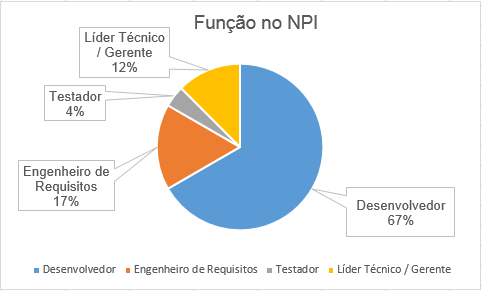
\includegraphics[scale=0.9]{./images/grafico-ci01}
\label{fig:grafico01-npi}
\legend {\fontsize{10}{12}\selectfont {Fonte: Elaborado pelo autor}.}
\end{figure}

A \autoref{fig:grafico01-npi} demonstra que a grande maioria dos estagiários do NPI estão alocados para atividades exclusivas de desenvolvimento, posteriormente atividade de engenharia de requisitos, líderes técnicos e gerentes. Este resultado obtido por meio das respostas ajudou a elucidar os conhecimentos e os tipos de conhecimentos predominante nos estagiários do núcleo.

\begin{figure}[H]
\centering
\caption[Conhecem Integração Contínua]{Conhecem Integração Contínua.}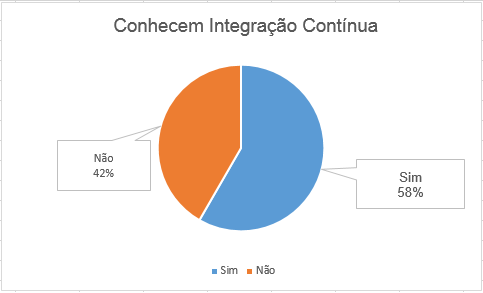
\includegraphics[scale=0.9]{./images/grafico-ci02}
\label{fig:grafico02-npi}
\legend {\fontsize{10}{12}\selectfont {Fonte: Elaborado pelo autor}.}
\end{figure}

Como descrito na \autoref{fig:grafico02-npi}, a maioria dos questionados conheciam o que era uma ferramenta de integração contínua, e como esta funcionava, embora esta não tenha sido uma superioridade notável, facilitou o processo de implantação em razão dos conhecimentos prévios dos estagiários a cerca do assunto, permitindo assim uma menor rejeição na implantação devido ao conhecimentos dos benefícios que este tipo de ferramenta causaria ao projeto.

\begin{figure}[H]
\centering
\caption[Utilização em Projetos Pessoais]{Utilização em Projetos Pessoais.}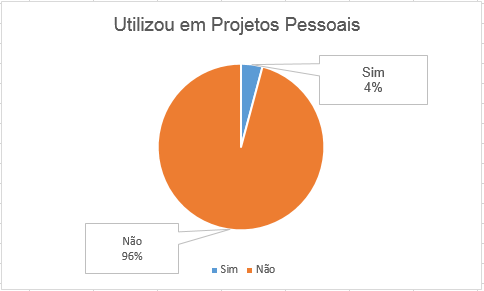
\includegraphics[scale=0.9]{./images/grafico-ci03}
\label{fig:grafico03-npi}
\legend {\fontsize{10}{12}\selectfont {Fonte: Elaborado pelo autor}.}
\end{figure}

Embora a maioria dos estagiários conheça a ferramenta, pouco mais de 4\% dos questionados utilizaram a integração contínua de forma prática, isto é, enfrentaram o impacto de sua utilização. Seja através do \textit{feedback} imediato fornecido pela ferramenta, ou pela alteração de seus processos de trabalho.	


\begin{figure}[H]
\centering
\caption[Conhecimento e Utilização de Ferramentas de Integração Contínua]{Conhecimento e Utilização de Ferramentas de Integração Contínua.}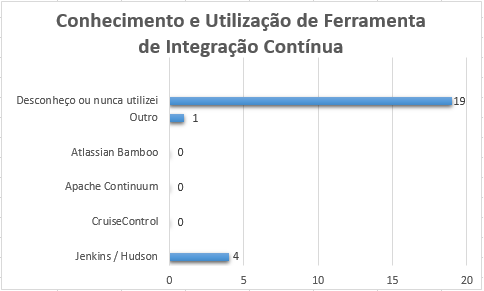
\includegraphics[scale=0.9]{./images/grafico-ci04}
\label{fig:grafico04-npi}
\legend {\fontsize{10}{12}\selectfont {Fonte: Elaborado pelo autor}.}
\end{figure}
O gráfico da \autoref{fig:grafico04-npi} contrasta com o gráfico anterior, onde a maioria desconhece ou nunca utilizou nenhuma ferramenta, e dentre a única ferramenta citada, o Jenkins / Hudson, enquanto um questionado citou outra ferramenta mas não especificou qual seria esta. De todo modo a familiarização de alguns questionados com a ferramenta facilitará o processo de aceitação desta por parte dos membros, e gerará uma unificação de conhecimento, pois todos os membros irão trabalhar e conhecer apenas uma ferramenta, no caso o Jenkins.

 

\begin{figure}[H]
\centering 
\caption[Conhecem Gerência de Configuração]{Conhecem Gerência de Configuração.}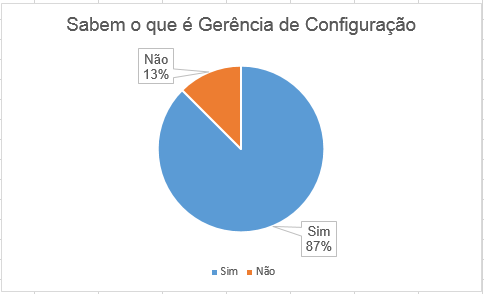
\includegraphics[scale=0.9]{./images/grafico-ci05}
\label{fig:grafico05-npi}
\legend {\fontsize{10}{12}\selectfont {Fonte: Elaborado pelo autor}.}
\end{figure}

Cerca de 87\% dos estagiários sabiam o que é uma atividade de gerência de configuração, sendo assim, supões-se que estes sabiam quais são as atribuições, responsabilidade e deveres exercidos por esta atividade. 

\section{Processo de Implantação da Ferramenta de Integração Contínua}\label{processoimpl}
Esta atividade tem como objetivo explicar como o processo ocorreu, apresentando o contexto do projeto, pontos negativos e positivos da implantação e aspectos a serem melhorados. A distribuição do conteúdo se dará da seguinte forma: \autoref{gpa} apresentará o projeto piloto onde a ferramenta foi implantada. O projeto GPA (Gestão de Projetos Acadêmicos).


\subsection{Gestão de Projetos Acadêmicos }\label{gpa}
O projeto GPA módulo de pesquisa tem como objetivo facilitar o processo de criação, submissão, aceitação e divulgação dos projetos da UFC do campus de Quixadá. Antes do desenvolvimento do sistema, este processo era totalmente manual. Enquanto este trabalho estava sendo desenvolvido o software do GPA era construído. Abaixo será descrito características deste sistema.

\begin{itemize}
	\item \textbf{Back-end:} A linguagem base da construção do sistema é o Java, com a utilização do Spring Framework. Este framework utiliza-se do padrão arquitetural MVC (Model View Control) além da rapidez de execução e segurança através da utilização do módulo de segurança Spring Security. A utilização do framework começou junto com a construção do sistema, sendo necessário treinamento aos membros das equipes, pois tratava-se de uma tecnologia nova no NPI.
	
	\item \textbf{Front-end:} Para a criação da aplicação front-end fora utilizado JSP (JavaServer Pages), HTML (HyperText Markup Language), CSS (Cascading Style Sheets) Javascript e o Bootstrap como framework front-end pois esta garante um padrão de interface na aplicação.
	
	\item \textbf{Build:} Para uma ferramenta de gestão de dependência e ferramenta de build, fora utilizado o Apache Maven, pois este garante que todos os membros do projetos tenham os mesmo itens de configuração corretos do projeto.
	
	\item \textbf{ORM - (Object-Relational Mapping):} O Hibernate é uma framework para realização do mapeamento objeto relacional com o objetivo de abstrair a persistência dos dados.
	
	\item \textbf{Gerenciamento de Projeto:} O Redmine foi a ferramenta utilizada para o gerenciamento do projeto durante a construção do sistema.
\end{itemize}

\subsection{Pontos Positivos}
\begin{itemize}
\item \textbf{Máquina com boas configurações:}A implantação ocorreu em uma máquina com boas configurações para hospedagem. A execução da ferramenta não sofreu engasgos ou problemas de lentidão devido a alta performance do hardware.

\item \textbf{Boa receptividade da equipe:}
Ao serem explanados de como a ferramenta atuava e quais eram seus benefícios para o projeto e produto, os membros da equipe não reagiram de maneira contrária à utilização da ferramenta, mesmo que esta alterasse seu processo de trabalho.

\item \textbf{Fácil entendimento:}
A ferramenta forneceu uma interface amigável que permitia o bom entendimento das ações que estavam sendo executadas, facilitando a interpretação dos dados por ela gerados.

\item \textbf{Coleta contínua de métricas:}
Através da integração do SonarQube como processo \textit{post-build} do Jenkins, o resultados das análises serviram de insumo para melhoria do código através de refatoração. Assim, uma alteração no processo do NPI ocorreu, de modo a contemplar uma atividades de correção de \textit{issues} fornecidas pelo SonarQube ao escopo da \textit{Sprint} afim de melhorar a qualidade do sistema, reduzir esforços e futuras manutenções. Além de permitir uma maior controle e acompanhamento do projeto, além de criar um entendimento da equipe de como construir o software daquele ponto em diante.

\item \textbf{Comunicação:}
Com a utilização da integração contínua percebeu-se que a comunicação da equipe melhorou, pois as informações de falha de \textit{build} foram discutidas assim que informadas aos responsáveis, que priorizavam sua correção, mesmo em horário fora de expediente.

\end{itemize}
\subsection{Pontos Negativos}

\begin{itemize}
\item \textbf{Ausência de um Gerente de Configuração:}
A ausência de um gerente de configuração com experiência na equipe foi sentida durante problemas com o repositório, gerando gastos no tempo da equipe e ociosidade na ferramenta. Embora em algum casos, o autor tenha ficado informalmente responsável por essas atividade perante equipe e projeto.

\item \textbf{Problemas estruturais:}
A execução da ferramenta em uma máquina de um dos laboratórios do NPI constantemente era desligada por algum funcionário da universidade, ou esta era desligada devido as constantes quedas de energia ocorridas, sendo necessário a reinicialização manual.

\item \textbf{Ausência de testes automatizados:}
A ausência de testes automatizados no projeto inviabilizou a valoração de um dos principais benefícios da integração contínua, que se trata da execução de testes em sua \textit{build} privada para verificação de problemas de integração, pois os testes embora fossem documentados e os casos de testes existissem, a forma como era testado era manual, através de teste de exploração.
\end{itemize}

\section{Métricas do Código}
A coleta das métricas do código foi realizado pelo SonarQube, onde este era um processo de \textit{post-build} da \textit{build} privada do Jenkins. Embora das muitas informações fornecidas pela ferramenta, apenas algumas foram bastantes focadas, como as \textit{issues} e linha de código duplicadas.

Após cada coleta, um histórico foi armazenado na base de dados da ferramenta, onde a última análise do dia foi mantida. O histórico das violações/\textit{issues} está mostrado na \autoref{fig:histissues}.

Neste percebe-se que, após a atribuição de um desenvolvedor para a atividade de solucionar as \textit{issues} existentes para o escopo da \textit{Sprint}, esta teve uma queda considerável, as violações tinham uma média em torno de 129 violações, e após este o processo de solução das \textit{issues}, esta teve uma queda para 87 e posteriormente, 81 violações. Uma queda de 38\%,  mesmo quando os outros membros da equipe continuaram a inserir código com violações.

\begin{figure}[H]
\centering 
\caption[Histórico de Violações]{Histórico de Violações.}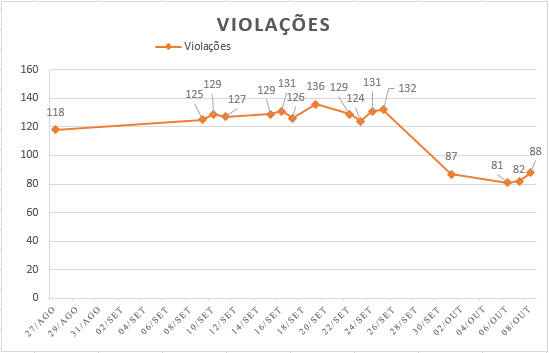
\includegraphics[scale=0.9]{./images/histviolacoes}
\label{fig:histissues}
\legend {\fontsize{10}{12}\selectfont {Fonte: Elaborado pelo autor}.}
\end{figure}	